\documentclass[UKenglish]{article}  %% ... or USenglish or norsk or nynorsk
\usepackage[latin1]{inputenc}         %% ... or utf8 or applemac
\usepackage[T1]{fontenc,url}
\usepackage{mathtools}
\usepackage{listings}
\lstset{
language=JAVA,
basicstyle=\small\sffamily,
numbers=left,
numberstyle=\tiny,
frame=tb,
columns=fullflexible,
showstringspaces=false
}
\usepackage{caption}
\usepackage{graphicx}
\urlstyle{sf}
\usepackage{babel,textcomp,csquotes,varioref,graphicx}
\usepackage{amsthm}

%\usepackage[backend=biber,style=numeric-comp]{biblatex}

\title{INF5040 Assignment 3}        %% ... or whatever

%\subtitle{Increasing QoE with SDN and NFV}         %% ... if any
\author{Ida Marie Froseth}                      %% ... or whoever

%\bibliography{mybib}                  %% ... or whatever

\begin{document}
%\ififorside{}
%\cleardoublepage{}
\maketitle{}
\cleardoublepage{}
\tableofcontents{}
\cleardoublepage{}
%\listoffigures{}
%\listoftables{}

\section{Introduction}


\subsection{Average path length}
\begin{figure}
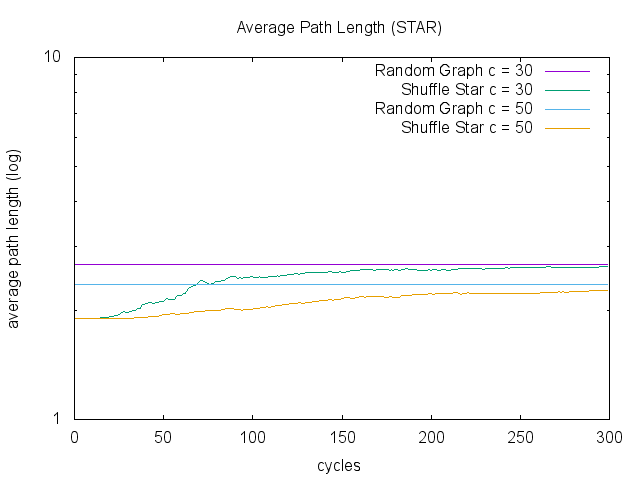
\includegraphics[scale=0.6]{plot/starPL.png}
	\caption{Star PL}
	\label{fig:starPL}
\end{figure}

\begin{figure}
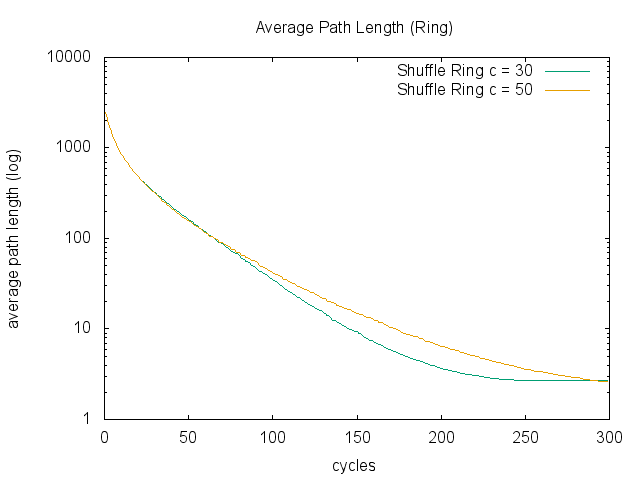
\includegraphics[scale=0.6]{plot/ringPL.png}
	\caption{Ring PL}
	\label{fig:ringPL}
\end{figure}


\subsection{Average clustering coefficient}

\begin{figure}
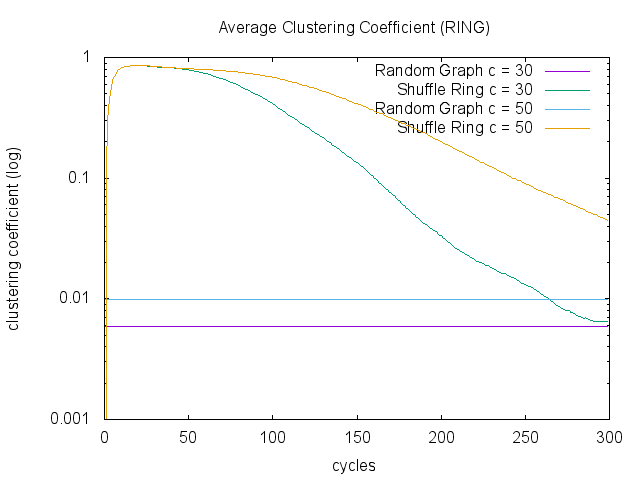
\includegraphics[scale=0.6]{plot/ringCC.png}
	\caption{Ring CC}
	\label{fig:ringCC}
\end{figure}

\begin{figure}
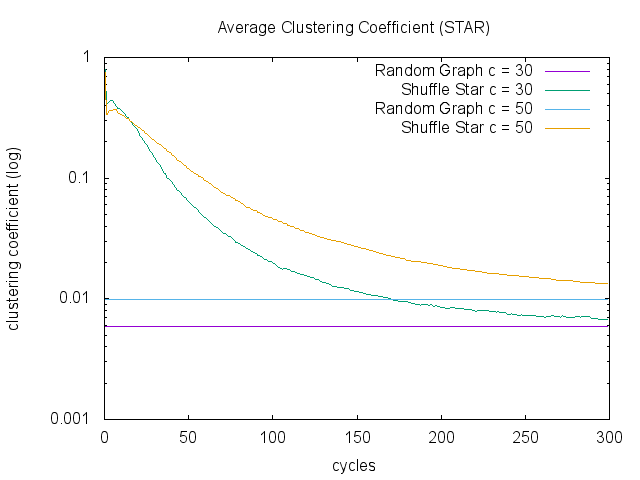
\includegraphics[scale=0.6]{plot/starCC.png}
	\caption{Star CC}
	\label{fig:starCC}
\end{figure}


\subsection{In-degree distribution}
\begin{figure}
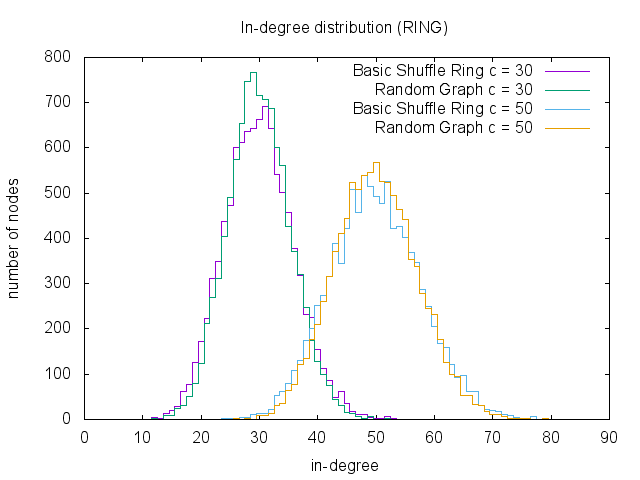
\includegraphics[scale=0.6]{plot/ringDD.png}
	\caption{Ring DD}
	\label{fig:ringDD}
\end{figure}

\begin{figure}
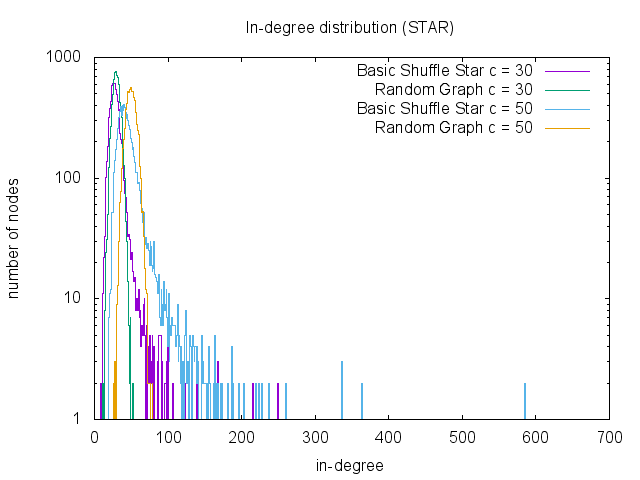
\includegraphics[scale=0.6]{plot/starDD.png}
	\caption{Star DD}
	\label{fig:starDD}
\end{figure}

\end{document}

